% LaTeX file for Chapter 02


\chapter{Data} 
Maybe it is the methods section. Here however, we give a couple hints.
Note that you can wisely use \rr{preamble}-chunks. Minimal, is likely: 

\bigskip

\section{Definitions}


% $T=time$
% $C=counts$
% $\lambda=\frac{C}{T}$
% \begin{tabular}{|c|c|c|c|c|}
%     \hline
%      & \textbf{Expectation} & \textbf{SD} & \textbf{Aleatory Uncertainty} & \textbf{Epistemic Uncertainty} \\ \hline
%     Point Estimate & $\lambda\cdot T$ & 0 & NO & NO \\ \hline
%     $C\sim Poi(\lambda)$ & $\lambda\cdot T$ & $\lambda\cdotT$ & YES & NO \\ \hline
%     $C\sim Poi(\Lambda)$ with $\Lambda\sim Gamma (\alpha,\beta)$& [...] & [...] & YES & YES \\ \hline
% 
% \end{tabular}



\hrule

\hrule
\bigskip

\textit{Target Population}

\bigskip
\hrule
\bigskip



\hrule

\bigskip 

This options are best placed in the main document at the beginning. Otherwise a \verb+cache=FALSE+ as knitr option is necessary to overrule a possible  \verb+cache=TRUE+ flag. 

\bigskip 

Notice how in Figure~\ref{f02:1} everything is properly scaled.   

\begin{figure}
\begin{knitrout}
\definecolor{shadecolor}{rgb}{0.98, 0.98, 0.98}\color{fgcolor}

{\centering 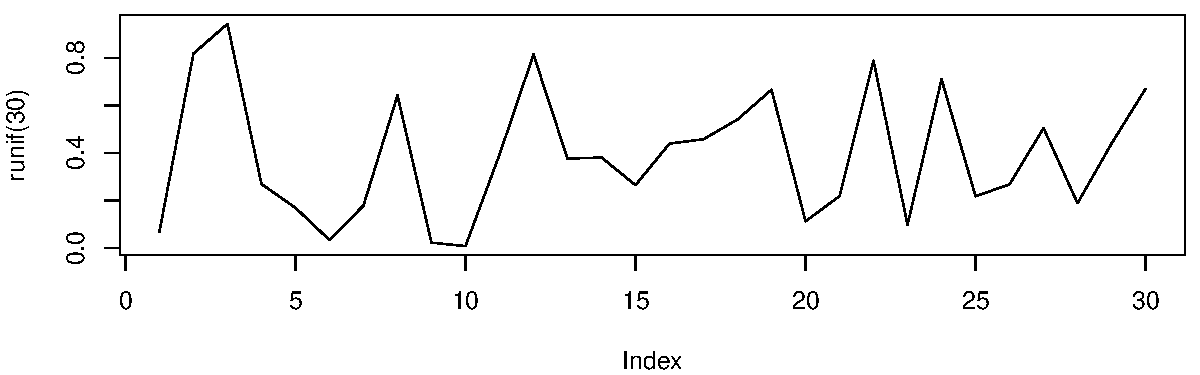
\includegraphics[width=\textwidth-3cm]{figure/ch02_figunnamed-chunk-3-1} 

}


\end{knitrout}
  \caption{Test figure to illustrate figure options used by knitr.}
  \label{f02:1}
\end{figure}


\section{Citations}

Recall the difference between \verb+\citet{}+ (e.g., \citet{Chu:Geor:99}), \verb+\citep{}+ (e.g., \citep{Chu:Geor:99}) and \verb+\citealp{}+ (e.g., \citealp{Chu:Geor:99}).
For simplicity, we include here all references in the file \verb+biblio.bib+ with the command \verb+\nocite{*}+.\nocite{*}

